\documentclass{article}
\usepackage[utf8]{inputenc}
\usepackage[parfill]{parskip}
\usepackage{graphicx}

\title{CS394R: Programming Assignment 1}
\author{Ashish Bora}
\date{September 2016}

\usepackage{hyperref}
\hypersetup{
    colorlinks=true,
    linkcolor=blue,
    filecolor=magenta,      
    urlcolor=cyan,
}

\begin{document}

\maketitle

\section{Introduction}

The setting for multi-armed bandit problem is as follows: There are $k$ actions we can take at any timestep. These are called arms of the bandit. We can choose any arm at a given timestep and pull it. As a result we receive a numerical reward chosen from a distribution (may not be stationary). Our objective is to maximize the expected total reward over time.

Given this environment, and objective we can design several algorithms/agents to solve it. \href{https://www.dropbox.com/s/b3psxv2r0ccmf80/book2015oct.pdf}{The textbook} describes greedy agent, $\epsilon$-greedy agent, UCB etc. These algorithms are deployed on a 10-arm testbed and their performance is compared.

We used \href{https://github.com/openai/gym}{OpenAIGym} for this assignment. Thus, the following were completed as a part of this assignment:
\begin{enumerate}
    \item Implement multi-arm bandit testbed as an OpenAIGym environment
    \item Implement $\epsilon$-greedy agent in OpenAIGym.
    \item Reproduce some plots from the book
    \item Test some agents in a non-stationary environment
    \item An experiment investiagting optimistic initializations.
\end{enumerate}

As discussed, three of us (myself, Ashwini Venkatesh and Kunal Lad) collaborated on the first two parts. The code for the same can be found in at \href{https://github.com/ashuven63/gym}{https://github.com/ashuven63/gym} (See recent commits). We also plan to open a Pull Request so that it can be integrated with the rest of the framework. This may be useful for beginners in reinforcement learning to play with environment parameters and agents.

The other parts of the assignment, including experiments and analysis were done individually.

\section{Multi Arm Bandit environment}

We implemented and registered the Multi Arm Bandit environment in OpenAIGym. Code for the same can be found \href{https://github.com/ashuven63/gym/blob/master/gym/envs/multiarm_bandit/multiarm_bandit.py}{here}.

The environment has the following configurable parameters:
\begin{enumerate}
    \item  Number of arms
    \item Mean and variance of the gaussian from which we pick $q_*$ values
    \item Variance of rewards around the $q_*$ values
    \item Whether the environment is stationary
    \item Variance of the random walk of $q_*$ values if we use non-stationary environment.
\end{enumerate}

In the stationary case, the $q_*$ values are sampled only once and then they remain fixed. In the non-stationary case, each $q_*$ value takes a random walk, i.e., at each timestep, random i.i.d. gaussian noise is added to each $q_*$ value.

\section{Epsilon Greedy Agent}

We implemented this as a python class. Code can be found \href{https://github.com/ashuven63/gym/blob/master/examples/agents/epsilon_greedy_agent.py}{here}.

The agent has the following configurable parameters:

\begin{enumerate}
    \item $\epsilon$
    \item Initialization value for $q_*$
    \item Weighting type: sample average or recency weighting
    \item $\alpha$ used if used recency weighting
\end{enumerate}

Note that with $\epsilon=0$, this is the same as the greedy agent. Optimistic initialization can be done by using high values for initialization of $q_*$.

Additionally, we also implemented several useful tools like state savers, print strings for easy debugging. Finally we have loggers and plotters to write stats to files and create plots from them.

\section{Experiments}

\subsection{Experiment 1 : Reproducing Fig. 2.2}

\textbf{Setup}
\begin{itemize}
    \item Environment setup: There are $10$ arms. $q_*$ values are sampled from zero mean, unit variance gaussian. Rewards are gaussian around $q_*$ value with variance $1$. The environment is stationary.
    \item Agents: We use three agents, with $\epsilon$ values $0$, $0.01$ and $0.1$ respectively. All of them use initial $q_*$ value of $0$ and use sample averaging. 
    \item We run each agent for $1000$ steps and $2000$ episodes. 
\end{itemize}

The results are in Fig. \ref{expt1}

\begin{figure}
    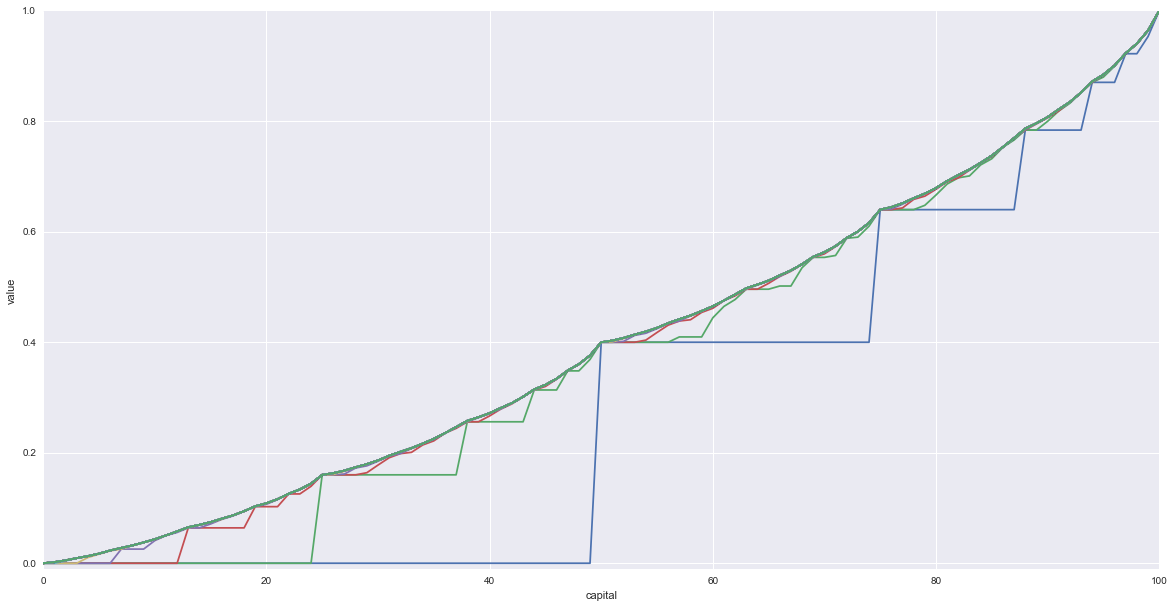
\includegraphics[width=\textwidth]{figure_1}
    \caption{Expt1}
    \label{expt1}
\end{figure}

\subsection{Experiment 2 : Reproducing Fig. 2.4}

\textbf{Setup}
\begin{itemize}
    \item Environment setup: Same as in the previous section.
    \item Agent1: Greedy agent with optimistic initial $q_*$ value of $5$. Recency weighting with $\alpha = 0.1$
    \item Agent2: $\epsilon=0.1$ with initial $q_*$ initial value of $0$. Recency weighting with $\alpha = 0.1$. 
    \item We run each agent for $1000$ steps and $2000$ episodes. Here are the results
\end{itemize}

The results are in Fig. \ref{expt2}. Note: The legend in the figure was incorrectly labeled with $\epsilon=0.01$).

\begin{figure}
    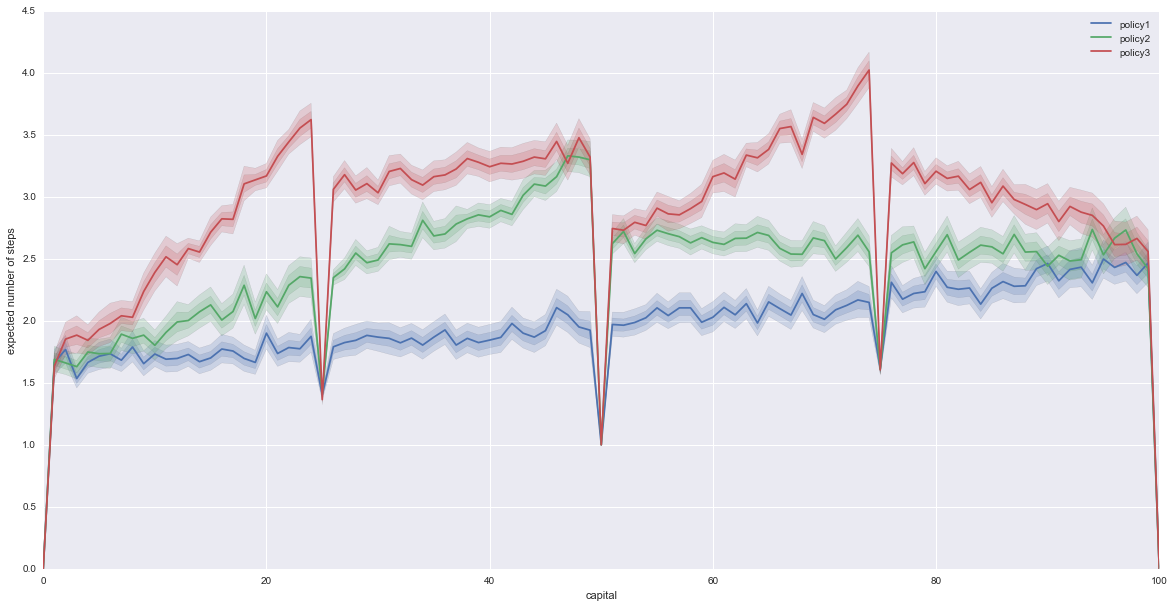
\includegraphics[width=\textwidth]{figure_2}
    \caption{Expt2}
    \label{expt2}
\end{figure}

\subsection{Experiment 3 : Exercise 2.3}

The task here is to see the performance of various agents on non-stationary environment. 

\textbf{Setup}
\begin{itemize}
    \item Environment setup is same as above, but additionally, at every step, to every $q_*$ value, we add a fresh sample of a gaussian random variable with variance $0.2$. (we call this random-walk-variance)
    \item Agent1: $\epsilon=0.1$, sample averaging
    \item Agent2: $\epsilon=0.5$, recency weighting with $\alpha=0.5$
    \item We run each agent for $2000$ steps and $1000$ episodes.
\end{itemize}

We can expect that the recency weighting should perform better than sample averaging because it gives more weight to the recent rewards. Large values of $\alpha$ and random-walk-variance were chosen to amplify this difference. 

Results can be seen in Fig. \ref{expt3}

\begin{figure}
    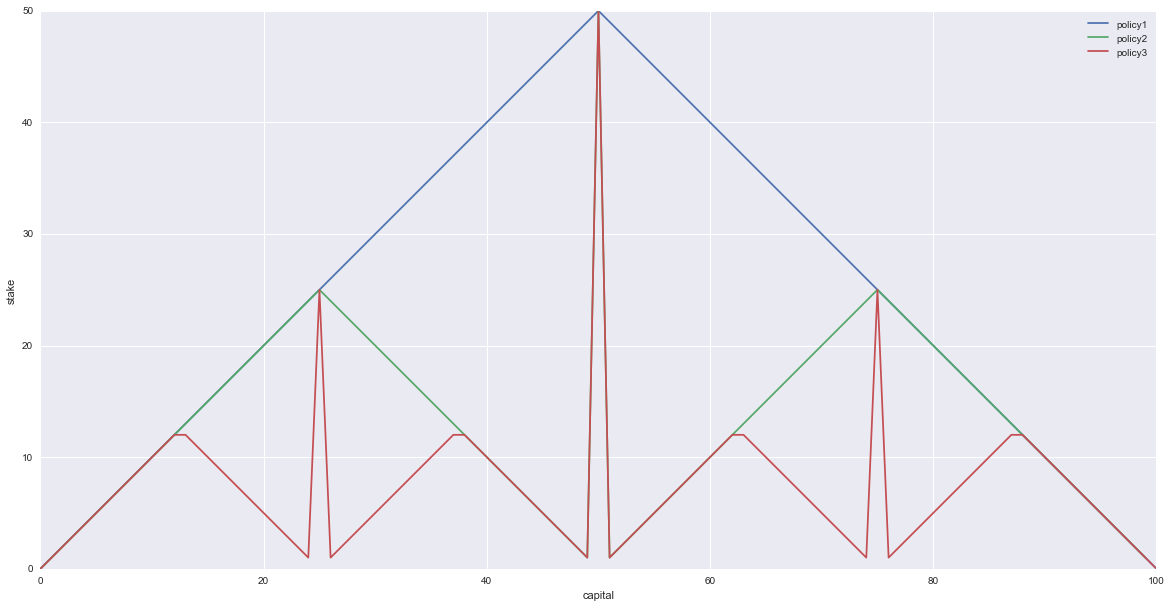
\includegraphics[width=\textwidth]{figure_3}
    \caption{Expt3}
    \label{expt3}
\end{figure}

This plot confirms that recency weighting significantly beats sample average method when used in a non-stationary environment.

\subsection{Experiment 4}

In Fig. 2.4 in the book, plot for optimistic initialization has a sharp peak at the $10$th time step (first pull at $t=0$). This is explained by the fact that the initial exploration due to optimistic values tries out all the arms one by one, and since the optimal arm pulls down the average the least, it is chosen with a large probability on the $10$th step. 

However, there is also a small peak after the first one, roughly around $20$. It was not clear to me if this is due to same kind of rotating exploration happening again, or due to some other factor. One simple way to test this is to vary the value of optimistic initialization. If the effect was due to rotating exploration encouraged by initialization, for larger values, we should see more peaks at every $10$th step. Also the sharpness of peaks should increase as the initialization value increases. Thus to test the hypothesis, I ran with the same setup as in Experiment $2$, but with different optimistic initializations. Results are in Fig. \ref{expt4}

\begin{figure}
    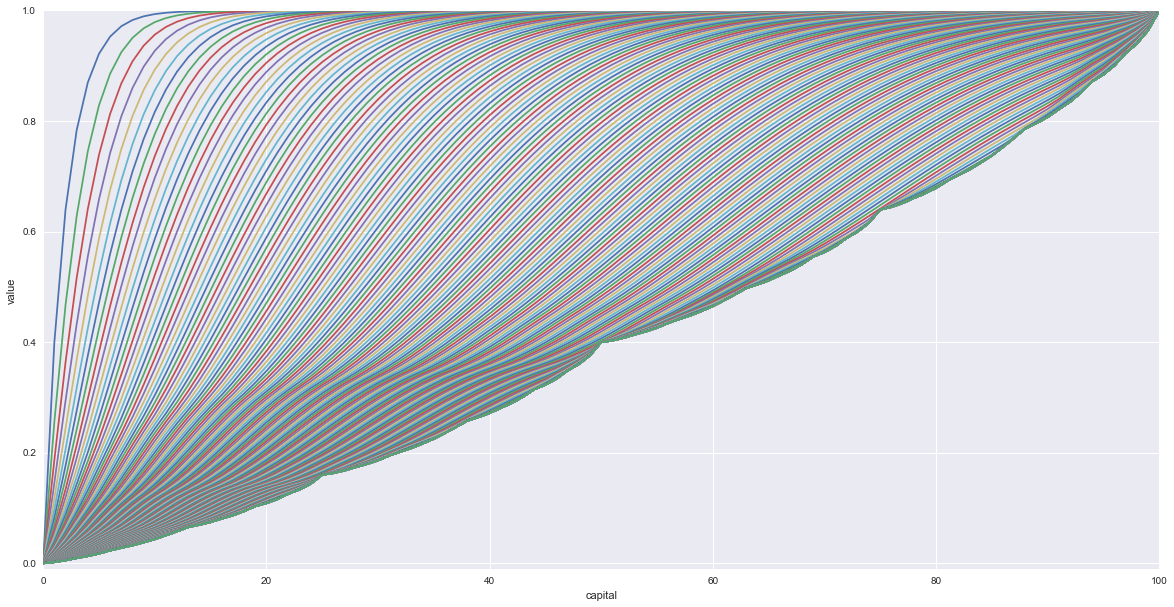
\includegraphics[width=\textwidth]{figure_4}
    \caption{Expt4}
    \label{expt4}
\end{figure}

We can see that many more peaks are observed and this confirms that the second smaller peak can indeed be attributed to optimistic initialization. Further we observe that after the initial spiky behaviour, the plot for percentage of times for which the optimal action was taken vs the number of timesteps steadily increases before stabilizing. Analyzing this further, we notice some more interesting findings:
\begin{enumerate}
    \item The effect of doubling optimism looks almost like shifting the graph to the right by a constant. One explanation for this is that it is harder to overcome wilder optimism than it is to overcome a less wild one. But since we are doing recency weighting, the initial value doesn’t matter too much after about 100 steps ($0.9^{100} \sim 2e-5$). So only the recent rewards from the arms would be used anyway, and hence they should perform well. In fact, higher the optimism, the more exploration would have happened and thus combined with recency weighting, we should have a better estimate of all values. Thus, with optimism, the graph should have risen earlier. What we see here is the opposite.
    \item The slope of increase for all three plots looks very similar. If the effect of initial value has died using recency weighting, this is what is expected. But, on the other hand, the delay in rise suggests that the effect has not died fully. Perhaps the interaction of initial values is through the number of times the arms are pulled rather than through entering the estimation of $q_*$ directly. But it is not clear to me exactly what is happening here.
\end{enumerate}

Full code for all experiments was not pushed to GitHub, because we wanted to do this individually. To generate the plots, I also modified logger, parser and plotter functions. Thus, some code is attached along with the report. Please see the README for details.

\end{document}
